\subsection{Giá trị thiếu và giá trị không hợp lệ}
\label{subsec:3_3_1}
Tập phát triển gốc có 2.399 dòng thiếu ít nhất một thuộc tính, chiếm 7,37\%. Giá trị thiếu chỉ xuất hiện ở các cột trong Bảng~\ref{tab:missing-train}. Một dòng có thể thiếu nhiều thuộc tính, nên tổng số ô thiếu không phải số dòng thiếu.

\begin{table}[htbp]
\centering
\small
\caption{Giá trị thiếu trên adult.data gốc}\label{tab:missing-train}
\begin{tabular}{lrr}
\toprule
Thuộc tính & Số ô thiếu & Tỷ lệ (\%) \\
\midrule
occupation & 1.843 & 5,66 \\
workclass & 1.836 & 5,64 \\
native-country & 583 & 1,79 \\
\bottomrule
\end{tabular}
\end{table}

\begin{figure}[htbp]
\centering
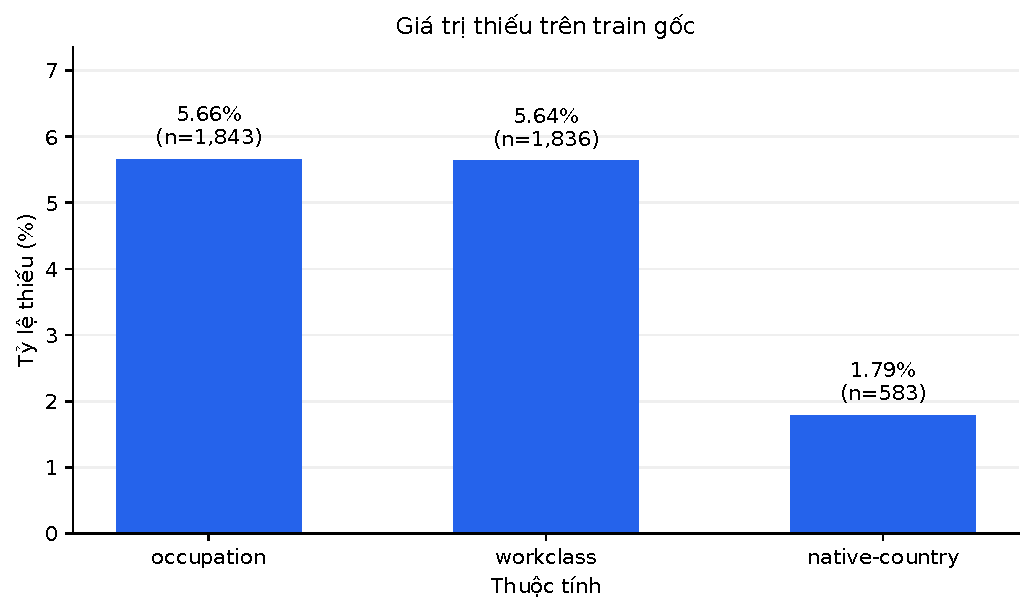
\includegraphics[width=.92\textwidth,height=.72\textheight,keepaspectratio]{Images/chapter_3/3_3/3_3_1/missing_values.pdf}
\caption{Tỷ lệ thiếu tính trên toàn bộ adult.data gốc}
\label{fig:missing-train}
\end{figure}

Các ký hiệu thiếu đã được nhận diện khi đọc dữ liệu. Việc lựa chọn cách điền thiếu sẽ được thực hiện trong pipeline và các giá trị điền được học từ train của từng lần chia, thay vì tính trước trên toàn bộ dữ liệu phát triển.
